%%%%%%%%%%% NO OLVIDAR COLOCAR ESTE COMENTARIO CON EL NUMERO DE EJERCICIO %%%%%%%%%%%%%
%%%%%%%%%%%%%%%%%%% EJERCICIO 3 %%%%%%
%%Text bf para negrilla , el \\ es para el salto de linea.
%%El primer \\ hace un espacio en el texto y el 2 \\ crea otro espacio
\textbf{Ejemplo 3}\newline
Se plantea la construcción de un puente y se han presentado dos proyectos, el primero es un puente colgante a un costo de 850.000.000 COP millones de pesos, cada año habrá que darle mantenimiento a la plataforma de asfalto a un costo de 3.000.000 COP millones de pesos, se estima que las reparaciones serán cada vez mayores y que éstas aumentarán de precio todos los años en 2.000.000 COP millones de pesos y cada 5 años habrá que cambiar los cables que sostienen el puente a un costo fijo de 100.000.000 COP millones de pesos, el segundo proyecto es un puente en concreto a un costo de 900.000.000 COP millones de pesos, cada 3 años habrá que reacondicionar las bases a un costo de 25.000.000 COP millones de pesos, el costo anual de mantenimiento se puede considerara fijo en 5.000.000 COP millones de pesos. Con una tasa del 24% determinar la mejor alternativa.

\textbf{Solución.}\\
\begin{center}

	\renewcommand{\arraystretch}{1.5}% Margenes de las celdas
	%Creación de la cuadricula
	\begin{longtable}{|c|c| }
		%Creamos una linea horizontal
		\hline
		%Definimos el color de la primera fila
		\rowcolor[HTML]{FFB183}
		%%%%% INICIO ASIGNACIÓN FECHA FOCAL %%%%%%%
		%%%%%%%%%% INICIO TITULO
		%Lo que se hace aquí es mezclar las 3 columnas en una sola
		\multicolumn{2}{|c|}{\cellcolor[HTML]{FFB183}\textbf{1. Asignación período focal}}   \\ \hline
		%%%%%%%%%% FIN TITULO
		%%%%% INICIO DECLARACIÓN DE VARIABLES %%%%%%%
		\multicolumn{2}{|c|}{$pf = 0 pmv$} \\ \hline
		%Definimos el color de la primera fila
		\rowcolor[HTML]{FFB183}
		%%%%% INICIO DECLARACIÓN DE VARIABLES %%%%%%%
		%%%%%%%%%% INICIO TITULO
		\multicolumn{2}{|c|}{\cellcolor[HTML]{FFB183}\textbf{2. Declaración de variables}}                                                                                   \\ \hline
		%%%%%%%%%% FIN TITULO
		%%%%%%%%%% INICIO DE MATEMÁTICAS
		$C_{A} = 850\,000COP$ & $C_{B} = 900\,000 COP$ \\
		$i_{A} = 24\% \text{ pav}$  & $i_{B} = 24\% \text{ pav}$ \\
		$\text{ }$ & $CAO_{B} =  5000000COP$\\
		$CAUE_{A} =  COP ?$ &   $CAUE_{B} =  COP ?$  \\ \hline
		%%%%%%%%%% FIN DE MATEMÁTICAS
		%%%%% FIN DECLARACIÓN DE VARIABLES


		%%%%% INICIO FLUJO DE CAJA
		\rowcolor[HTML]{FFB183}
		\multicolumn{2}{|c|}{\cellcolor[HTML]{FFB183}\textbf{3. Diagrama de flujo de caja}}                                                                                  \\ \hline
		%Mezclamos 3 columnas y pondremos el dibujo
		%%%%%%%%%%%%% INSERCIÓN DE LA IMAGEN
		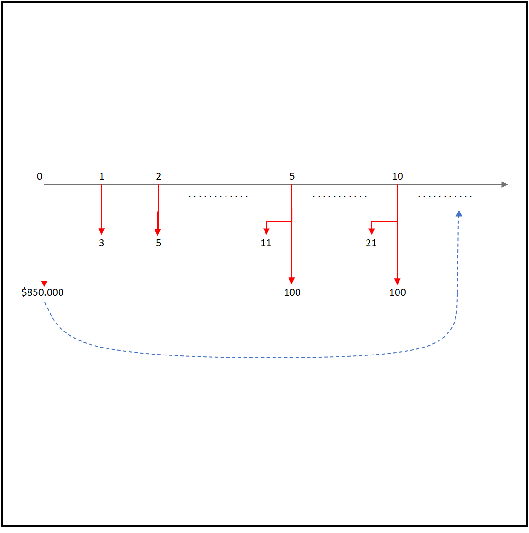
\includegraphics[trim=-5 -5 -5 -5 , scale=0.7]{10_Capitulo/ejemplos/3/Capitulo10Ejercicio3a.pdf} &    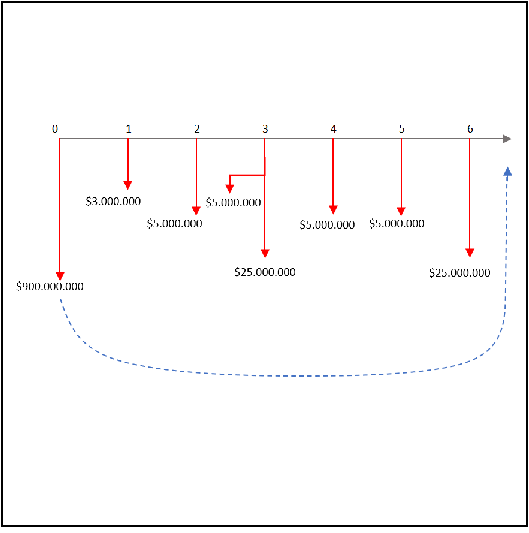
\includegraphics[trim=-5 -5 -5 -5 , scale=0.7]{10_Capitulo/ejemplos/3/Capitulo10Ejercicio3b.pdf}\\ \hline
		%%%%%%%%%%%%% FIN INSERCIÓN DE IMAGEN
		%%%%%FIN FLUJO DE CAJA

		%%%%% INICIO DECLARACIÓN FORMULAS
		%%%%%%%%%%% INICIO TITULO
		\rowcolor[HTML]{FFB183}
		\multicolumn{2}{|c|}{\cellcolor[HTML]{FFB183}\textbf{4. Declaración de fórmulas}}                                                                                    \\ \hline
		%%%%%%%%%%% FIN TITULO
		%%%%%%%%%%% INICIO MATEMÁTICAS

		$VP=\frac{R}{i} \text{ Valor presente}$  &        $CAUE=VPN\bigg[\frac{i(1+i)^{n}}{(1+i)^{n}-1}\bigg]$                                                  \\ \hline
		%%%%%%%%%% FIN MATEMÁTICAS
		%%%%%% INICIO DESARROLLO MATEMÁTICO
		\rowcolor[HTML]{FFB183}
		%%%%%%%%%%INICIO TITULO
		\multicolumn{2}{|c|}{\cellcolor[HTML]{FFB183}\textbf{5. Desarrollo matemático}}                                                                                      \\ \hline
		%%%%%%%%%% FIN TITULO
		%%%%%%%%%% INICIO MATEMÁTICAS
		44.000.000$=\frac{X}{0.24}$ &  $CAUE_{B} =  11.000.000 COP + 12.180.000 COP$ \\
		$X= 11000000 COP$ & $+ 5.000.000 + 22.500.000 + 6.560.000 $\\
		$100000000=\frac{Y}{0.25}$ & $+ 5.000.000=   236.560.000 COP$\\
		$Y=  12.800.000 COP$ & \\
		$850000000=\frac{Z}{0.25}$ & \\
		$Z=  212.500.000 COP$ & \\
		$CAUE_{A}=11.000.000+12.800.000$ &\\ 
		$+212500000= 235.680.000 COP$ &                         \\ \hline
		%%%%%%%%%% FIN MATEMÁTICAS
		%%%%%% FIN DESARROLLO MATEMÁTICO

		\rowcolor[HTML]{FFB183}
		\multicolumn{2}{|c|}{\cellcolor[HTML]{FFB183}\textbf{6. Respuesta}}    \\ \hline

		\multicolumn{2}{|c|}{El CAUE para el proyecto uno es de 235.680.000 COP y el CAUE para el} \\ 
		\multicolumn{2}{|c|}{proyecto dos es de 236.560.000 COP. Ya que el proyecto uno es menor } \\ 
		\multicolumn{2}{|c|}{que el proyecto dos, el contratista debería elegir el proyecto uno.}\\ \hline
		
	\end{longtable}
	%Se crean dos lineas en blanco para que no quede el siguiente texto tan pegado
	%\newline \newline
\end{center}
%%%%%%%%%%%%%%%%%%%%%%%%%%FIN EJERCICIO X %%%%%%%%%%%%%%%%%%%%%%%%%%%
